\documentclass[a4paper,usenatbib]{aspdoc}
\usepackage{newtxtext,newtxmath}
\usepackage{ae,aecompl}
\usepackage{graphicx}	% Including figure files
\usepackage{amsmath}	% Advanced maths commands
\usepackage{amssymb}	% Extra maths symbols
\usepackage{lipsum}
\usepackage{float}
\usepackage{multirow}
\usepackage{booktabs}
\usepackage{geometry}
\geometry{left=25mm,right=25mm,top=25mm,bottom=25mm}

\usepackage[load=prefixed]{siunitx}
\sisetup{output-decimal-marker = {,}}

\newcounter{simplecount}
\setcounter{simplecount}{0}
\renewcommand{\theequation}{\arabic{simplecount}}
\newcommand{\owncount}{\refstepcounter{simplecount}}

% Title
\title[]{VAK: Vakuum}

% The list of authors
\author[]{
    Riedel Lisa, Wegmann Peter
    \newauthor
    \,Gruppe 6
}

% Don't change these lines
\begin{document}
    \label{firstpage}
    \pagerange{\pageref{firstpage}--\pageref{lastpage}}
    \maketitle
    
    

    % Body
    \section{Einleitung}\label{sec:intro}
                Bei diesem Versuch wurden einfache Vakuumstechniken durchgeführt und die Eigenschaft von idealen Gasen untersucht. Luft wurde dabei näherungsweise als ideales Gas angenommen.
                
        \subsection{Einführende Fragen}
                Im den folgenden 3 kleineren Kapitel werden drei theoretische Fragen gestellt und konkret beantwortet.
            
            \subsubsection{Strömungen}
                Die Strömung von Gasen erfolgt durch die thermische Bewegung einzelner Gasteilchen als auch aufgrund makroskopischer Kräften infolge eines lokalen Druckunterschiedes. Das Verhalten der Strömung wird durch Trägheitskräfte, Reibungskräfte und Druckkräfte bestimmt. Bei Gasen wird die Gewichtskraft meist vernachlässigt.\\
                Im Folgenden werden die charakteristischen Eigenschaften der molekularen und viskosen Strömung aufgeführt.\\
                Die \textbf{molekulare Strömung} wird durch die thermische Bewegung der Gasteilchen angetrieben. Da die mittlere freie Weglänge der Teilchen sehr groß im Vergleich zur Querausdehnung der Leitung ist, kommen gegenseitige  Teilchenstöße fast nicht mehr vor. Dies ist bei genügend kleinem Druck gegeben. Infolgedessen bewegen sich die Teilchen unabhängig voneinander. Durch häufige Stöße mit der Leitungswand ergibt sich dann ein Zickzackkurs. Das makroskopische Strömungsverhalten ergibt sich durch die Bahnen vieler einzelner Teilchen. \\
                Die \textbf{viskose Strömung} oder Kontinuums-Strömung wird durch einen lokalen Druckunterschied angetrieben. Die mittlere freie Weglänge der Teilchen ist viel kleiner als der Leitungsquerschnitt. Das passiert bei genügend hohem Druck. Das bedeutet, dass die Teilchen sehr oft gegeneinander stoßen. Dabei findet ein ständiger Austausch von Impuls und Energie statt. \cite{Vaktech}
            
            \subsubsection{Druck 1}
                Unter Verwendung eines Schlauches mit Durchmesser \SI{25}{\milli\metre} und Länge \SI{65}{\cm} und einer Kapillare mit Durchmesser \SI{1}{\milli\metre} und einer Länge l = \SI{9,5}{\cm} berechnet man den Druck innerhalb des Rezipienten mit einem Volumen von \SI{3}{\litre} nach 10 Minten folgendermaßen.\\
                Es wird angenommen, dass innerhalb des Zeitintervalls kein Wechsel zwischen viskosem und molekularen Bereich stattfindet. Zuerst wird der Leitwert der Kapillare mit Hilfe von Formel \ref{eq:lvs} berechnet. Danach wird das effektive Saugvermögen mit der Formel \ref{eq:seff} berechnet. Der Leitwert des Schlauches im viskosem Bereich wird aus Tabelle \ref{tab:theoleit} abgelesen. Damit ergibt sich sein ein effektives Saugvermögen von \SI[per-mode = fraction]{0,026}{\cubic\metre\per\hour} im viskosem Bereich. Für das Saugvermögen wurde die Herstellerangabe von \SI[per-mode = fraction]{3,7}{\cubic\metre\per\hour} verwendet. Zur Überprüfung wird nun die Zeit bis ein Druck von \SI{1}{\hecto\pascal} erreicht wird mit der Formel \ref{eq:pressure} berechnet. Als Ergebnis erhält man $0,79 h \approx 47 min$. Damit findet kein Wechsel zwischen vikoser und molekularer Strömung innerhalb des Zeitintervalls statt. Nun kann mit der selben Formel der Druck nach 10 Minuten berechnet werden. Dieser Beträgt nach $10 min \approx 0,167 h$ etwa \textbf{\SI[detect-weight]{225,79}{\hecto\pascal}}.
            
            \subsubsection{Druck 2}
                Das beste im Labor erzeugte Vakuum enthielt noch 1 Molekül pro $\mathrm{m}^3$.\\
                Der Druck kann mittels der Gleichung \ref{eq:idpressure} ermittelt werden. Dabei wird eine Temperatur von \SI{20}{\degreeCelsius}\, also \SI{293}{\kelvin} angenommen. Man erhält einen Druck von etwa \textbf{ \SI[detect-weight]{4,04e-24}{\pascal}}. Da nur noch sehr wenige Teilchen vorhanden sind, die mit der Messapparatur wechselwirken können, ist eine Druckmessung in diesem Bereich nur sehr schwer möglich.
                
            
       
    \section{Verwendete Methoden}\label{sec:method}
        Als ideales Gas bezeichnet man ein Gas, dessen Teilchen als Kugeln betrachtet werden und diese nur über elastische Stöße miteinander wechselwirken. Über die Zustandsgleichung der idealen Gase können dann der Druck $p$ in Pascal, die Temperatur $T$ in Kelvin, das Volumen $V$, die Teilchenzahl $N$ und die universelle Gaskonstante, auch Boltzmannkonstante genannt, $k_B = 1,38 \cdot 10^{-23}$ miteinander verknüpft werden. 
        \begin{equation}
            \owncount
            p\cdot V = N k_{B}T
            \label{eq:idpressure}
        \end{equation}\\
                Die Saugleistung bei der im Versuch verwendeten Pumpe ist über einen weiten Druckbereich proportional zum Druck. Daher kann das Saugvermögen $S$ mit folgender Formal berechnet werden. 
        \begin{equation}
            \owncount
            S = -\frac{1}{p}\frac{d(Vp)}{dt}
            \label{eq:saug}
        \end{equation}\\
                Handelt es sich bei der Änderung des Volumens mit der Zeit um einen linearen Vorgang kann die Formel folgendermaßen vereinfacht werden.\\
        \begin{equation}
            \owncount
            S = -\frac{p_0}{p}\cdot\frac{\Delta V}{\Delta t}
            \label{eq:saugl}
        \end{equation}\\
                In der Regel kann das volle Saugvermögen nicht ausgenutzt werden, da kleine Leitwerte von Rohren und Engstellen es reduzieren. Für das effektive Saugvermögen $S_{eff}$ gilt also
        \begin{equation}
            \owncount
            S_{eff} = \left(\frac{1}{S}+\frac{1}{L_1}+\frac{1}{L_2}+...\right)^{-1}
            \label{eq:seff}
        \end{equation}\\
                Wobei $L_{1,2,...}$ die Leitwerte der hintereinander geschalteten Verbindungsstücken ist.\\
                $S_{eff}$ ist in der Regel kein konstanter Wert, da für viskose Strömung die Leitwerte nach Formel \ref{eq:lvs} vom Druck abhängen. Betrachtet man jedoch nur kleine Bereiche, kann $S_{eff}$ als konstant angenommen werden und der Druck in dem Bereich mit folgender Formel berechnet werden.
        \begin{equation}
            \owncount
            p(t) = p_0 \cdot \exp{\left(\frac{-S_{eff}}{V}\cdot t\right)}
            \label{eq:pressure}
        \end{equation}\\
                $p_0$ ist hierbei der in dem Bereich herrschende Druck.\\
                Zur Ermittlung der experimentellen effektiven Saugleistung wird Gleichung \ref{eq:pressure} folgendermaßen umgestellt. 
        \begin{equation}
            \owncount
            S_{eff} = \left(\kappa -\frac{\log(p_0)}{t}\right)\cdot V\cdot 3,6
            \label{eq:seffExp}
        \end{equation}\\
        Hierbei beschreibt $\kappa = \frac{\log(p(t))}{t}$ die Steigung der Funktion. Der $\frac{\log(p_0)}{t}$ Term ist ein konstanter Faktor. Die Zeit $t$ und die Steigung kann aus dem Graphen aus Abbildung \ref{fig:saugEff} abgelesen werden. Für die effektive Saugleistung im molekularen Bereich vereinfacht sich die oben genannte Formel, da sie unabhängig vom im Bereich herrschenden Druck ist, zu folgender Form.
        \begin{equation}
            \owncount
            S_{eff} = \kappa \cdot V \cdot 3,6
            \label{eq:seffExpM}
        \end{equation}\\
            Zur Ermittlung der theoretischen effektiven Saugleistung werden die Leitwerte der Rohre benötigt. Diese sind vom Bereich der Strömung abhängig. Bei viskoser Strömung berechnen sich diese aus nachfolgender Gleichung.
        \begin{equation}
            \owncount
            L = \frac{\pi\cdot d^4}{128\cdot\eta\cdot l}\cdot\overline{p}
            \label{eq:lvs}
        \end{equation}\\
                $L$ ist der zu berechnende Leitwert, $d$ der Druchmesser des Rohres, $\eta$ die Viskosität des Gases, $l$ die Länge des Rohres und $\overline{p}$ der mittlere Druck des Gases. Bei den Berechnungen wird hierfür der Wert \SI{500}{\hecto\pascal} angenommen.\\
                Bei niedrigen Drücken ist die oben aufgeführte Formel nicht mehr gültig. Daher wird die nachfolgende Formel für molekulare Strömungen verwendet.
        \begin{equation}
            \owncount
            L = \sqrt{\frac{\pi \cdot k_B \cdot T}{18 \cdot m}}\cdot \frac{d^3}{l}
            \label{lms}
        \end{equation}\\
                Hierbei ist $m$ die Molekülmasse. Für Luft bei \SI{20}{\degreeCelsius}\, ergibt sich dann folgende Formel.
       \begin{equation}
            \owncount
            L = 121 \frac{m}{s} \cdot \frac{d^3}{l}
            \label{eq:leitwert}
        \end{equation}\\
        Soll auch die die Leistung $P$ des Pirani-Vakuummeter berechnet werden, so kann folgende Formel verwendet werden.
        \begin{equation}
        \owncount
            P = \frac{1}{4}\cdot R \cdot I^2
            \label{eq:power}
        \end{equation}
        Da sich das Pirani-Vakuummeter in einer Brückenschaltung mit \SI{50}{\ohm} Widerständen befindet, setzt man R = \SI{50}{\ohm} fest. Der Strom $I$ wird vom Manometer abgelesen.
    
    
    \section{Experimentelles Vorgehen}\label{sec:experiment}
            Um sinnvolle Werte bei dem verwendeten Pirani-Vakuummeter zu erhalten wurde dies zuerst über das Referenzvakuummeter kalibriert. Dabei wurden Drücke im Bereich von \SI{e-2}{\hecto\pascal} bis \SI{e3}{\hecto\pascal} angenommen. Zu dem Druck wurde die Stromstärke des Manometers abgelesen, um später eine Kalibrierkurve zu erstellen.\\
            Danach wurde das Saugvermögen mit Hilfe eines Kolbenprobers bestimmt. Dabei wurde das Manometer an die Pumpe angeschlossen. Der Kolbenprober wurde über einen Dreiwegehahn und einem Gummischlauch an der Pumpe angeschlossen. Bei diesem Versuch wurden zu 4 verschiedenen Drücken die Zeit, in der ein Volumen von $\Delta V = $\SI{80}{\milli\litre} verdrängt wurde, gemessen. Diese Messung wurde drei mal wiederholt. Es wurde der Druck und das Zeitintervall notiert.\\
            Beim letzten Versuch sollte das effektive Saugvermögen der Pumpe untersucht werden. Hierfür wurde die Pumpe mit einem Schlauch oder einem Schlauch mit Kapillare an einen Rezipienten angeschlossen. Der Druck wurde mit dem Manometer am Rezipienten über die gemessene Stromstärke bestimmt. Abhängig von der Kapillare wurde unterschiedlich lange vakuumiert. Zu bestimmten Zeitabständen wurde dann der Druck notiert.  
    
    
    
    \section{Ergebnisse}\label{sec:result}
        \subsection{Kalibrierkurve}
            Um das Pirani-Vakuummeter zur Druckmessung nutzen zu können, müssen die Daten aus dem Kalibriervorgang erst ausgewertet werden. Dies folgt daraus, dass dieses lediglich Strom $I$ anzeigt. Kombiniert man nun die Referenzwerte mit dem angezeigten Strom, so erhält man eine S-förmige Kurve durch doppellogarithmische Auftragung. Dies ist in Abbildung \ref{fig:calibration}a sehr gut zu sehen. Aufgrund weniger Datenpunkte im Bereich von 10 - 100 mbar wurde eine Funktion gefittet. Diese ermöglicht eine genaue Verwendung des Pirani-Vakuummeter.\\
            Aufgrund der doppellogarithmischen Auftragung von $P$ gegen $p$, erhält aufgrund der in Gleichung \ref{eq:power} quadratischen Abhängigkeit von $I$ zu $p$ eine Gerade in Abbildung \ref{fig:calibration}b\footnote{Der Sourcecode zur Berechnung der Ergebnisse und Fehler findet sich unter \url{https://github.com/Wegii/AP2-SS19}\label{note:source}}.
            
            \begin{figure*}
                \centering
                
                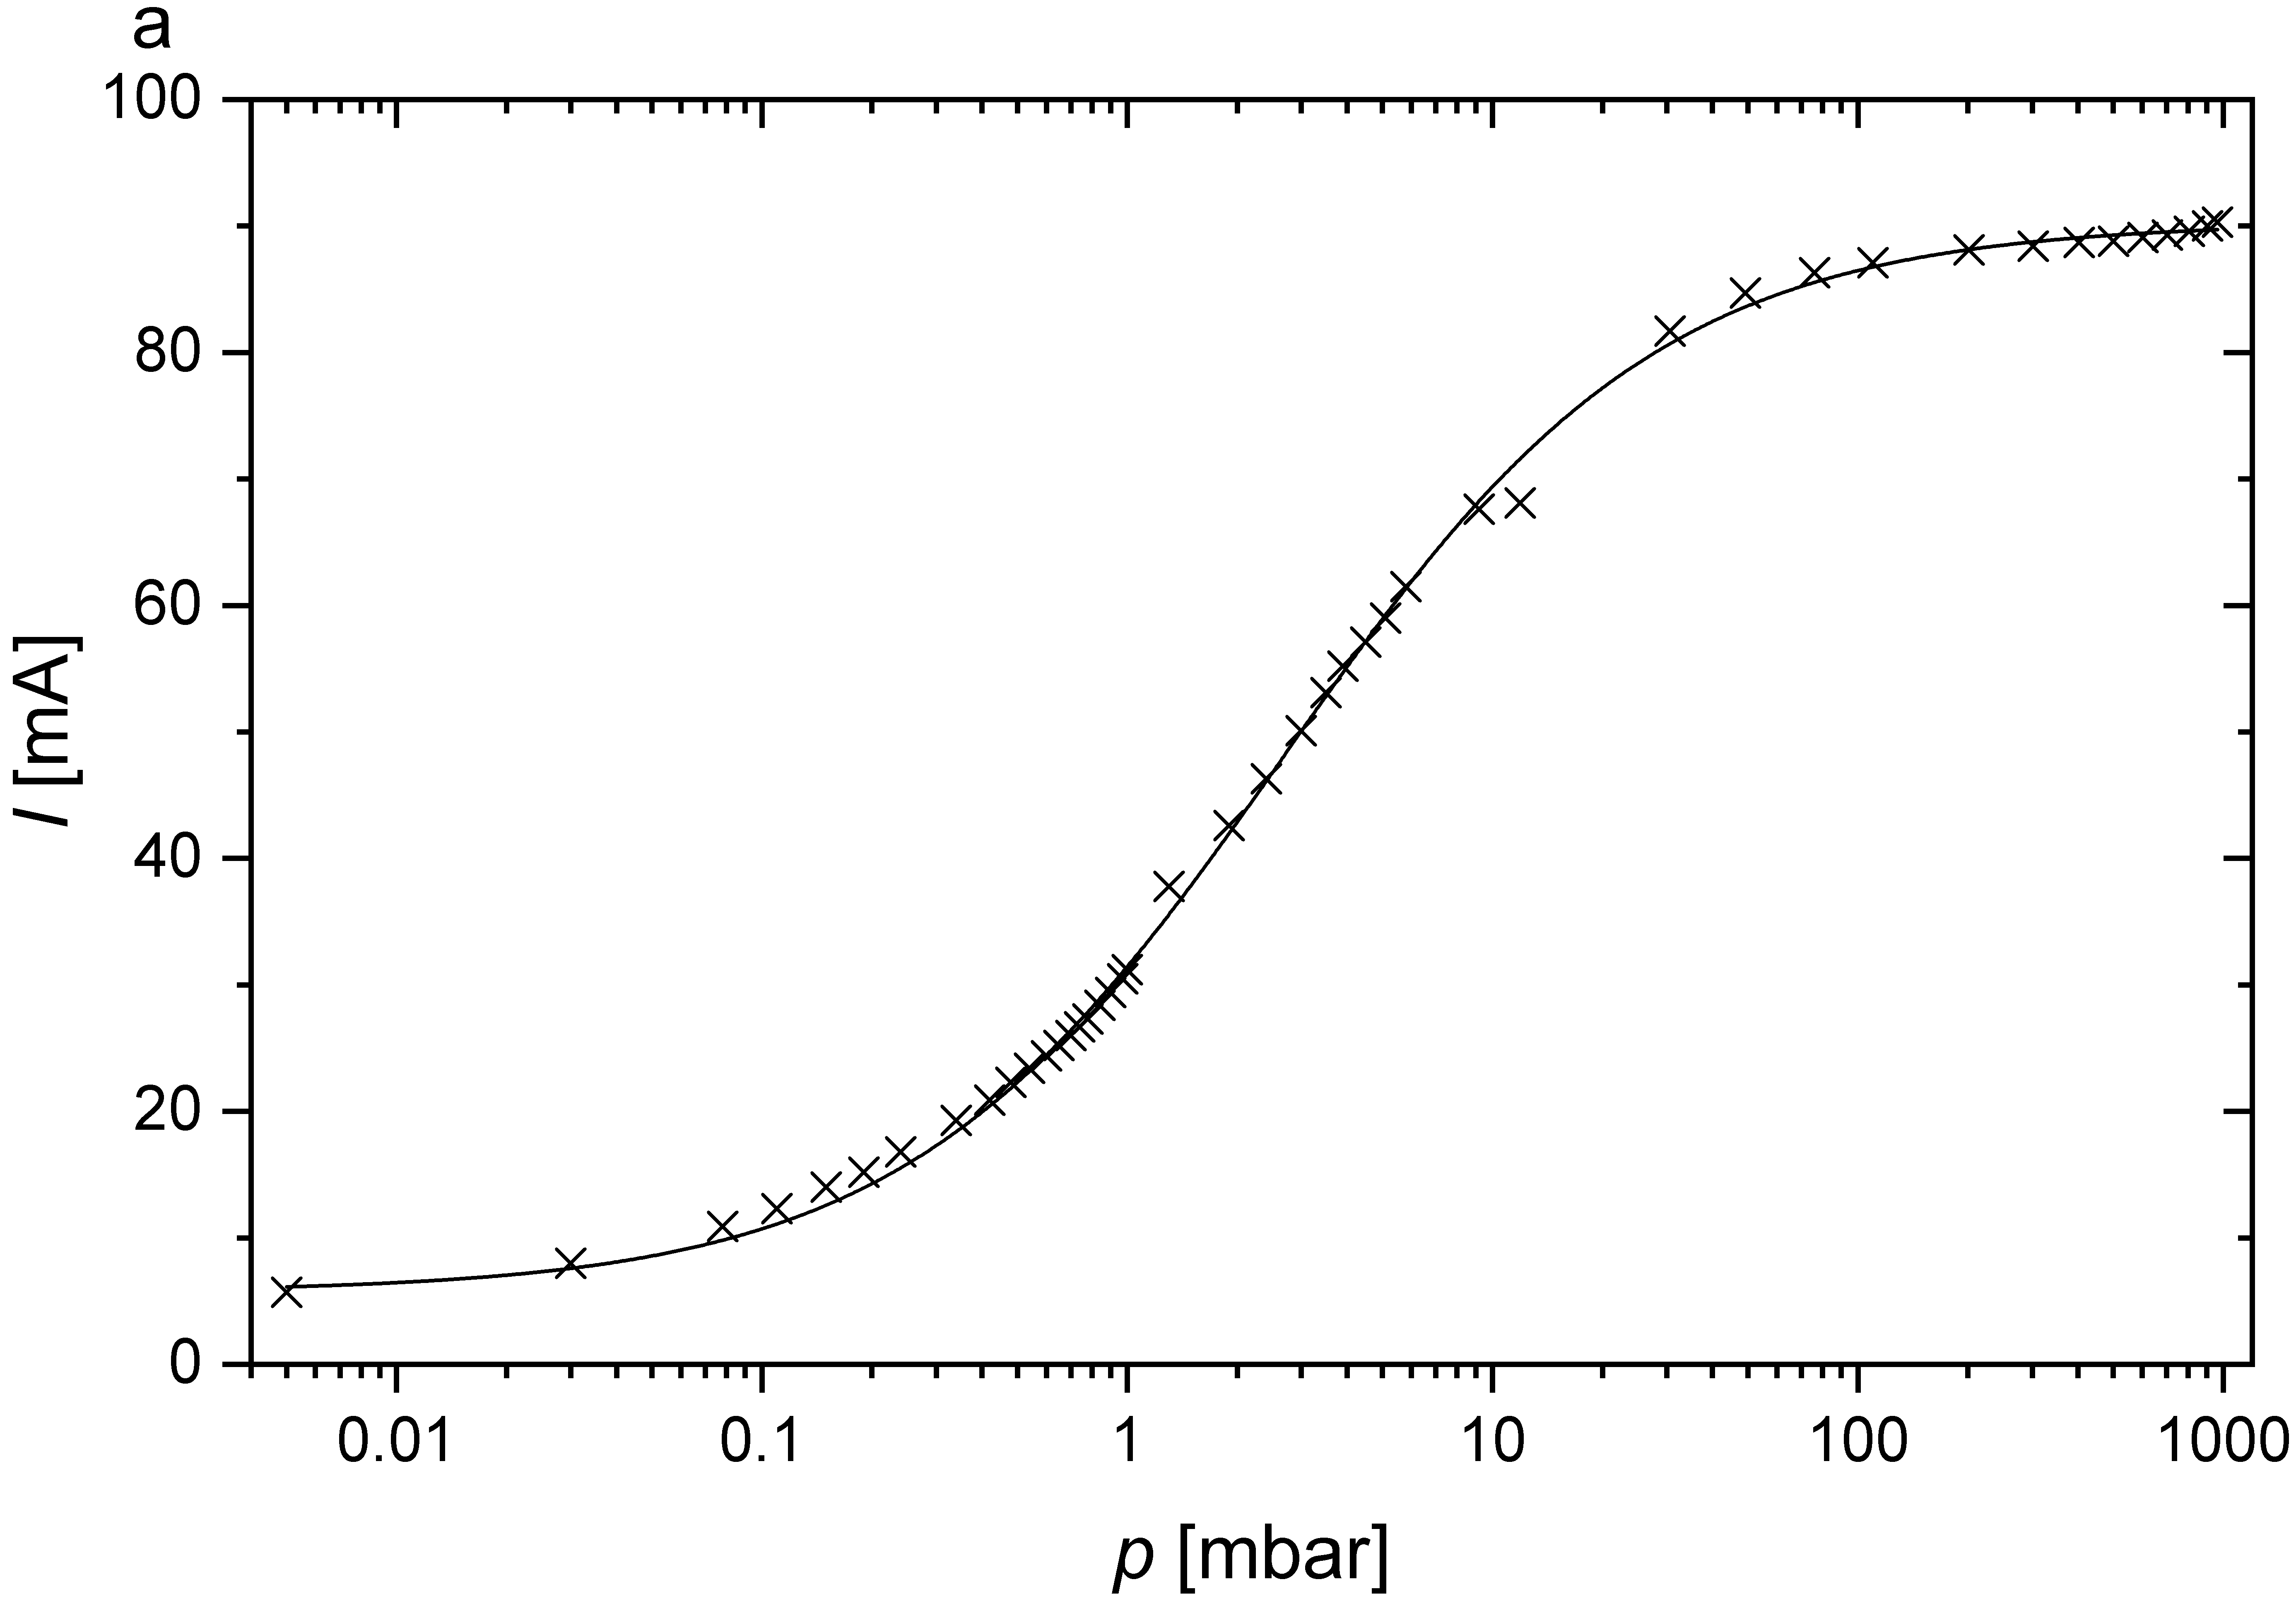
\includegraphics[width=110mm]{graphs/kalibStrom1.png}
                
                \hspace{.15cm}
                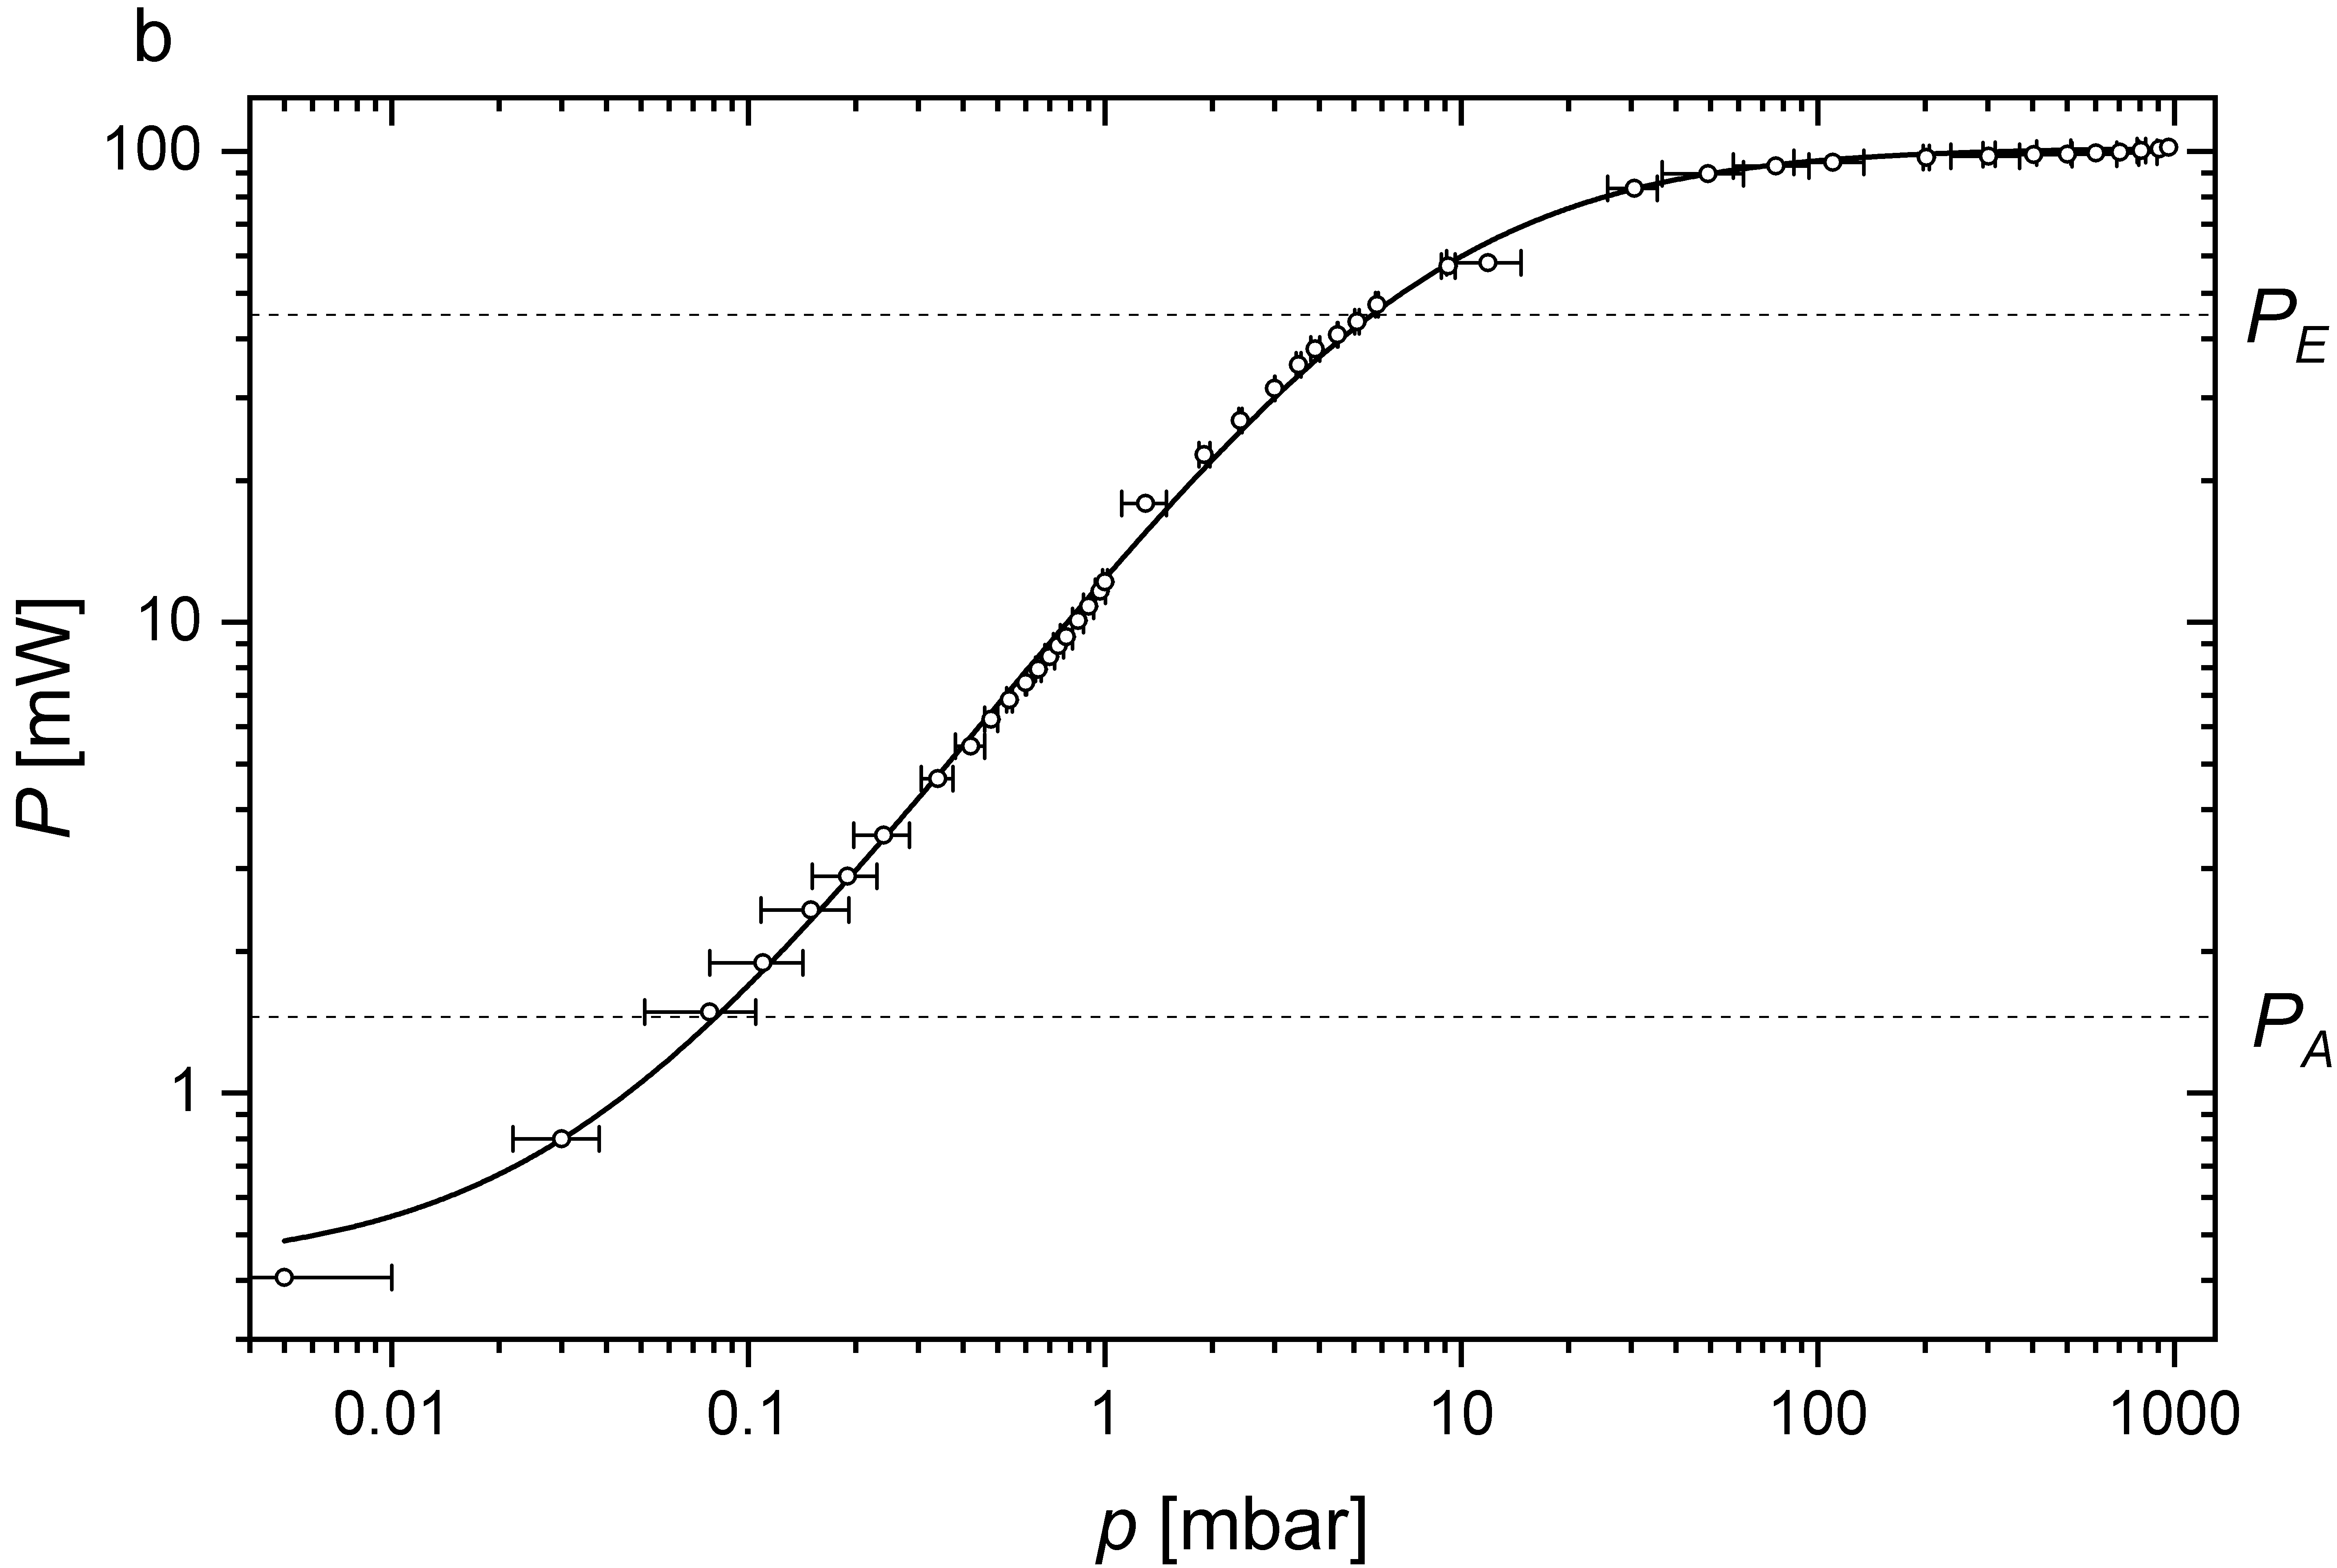
\includegraphics[width=115mm]{graphs/kalibLeistung1_fit.png}
                
                \caption{
                    \textbf{a} Doppellogarithmische Auftragung des gemessenen Strom $I$ gegen den Druck $p$. Hierbei handelt es sich um die Kalibrierkurve des Pirani-Vakuummeter, durch welcher der Druck abgelesen werden kann.
                    \textbf{b} Doppellogarithmische Auftragung der Leistung $P$ des Pirani-Vakuummeter gegen den Druck $p$. $P_A = 1.45$ mW markiert den Anfang, bei dem die Leistung linear mit dem Druck ansteigt. $P_E = 45$ mW markiert das Ende dieses linearen Zusammenhangs. \\
                    Beide Funktionen in \textbf{a} und \textbf{b} dienen als \textit{guide for the eye}.
                }
                \label{fig:calibration}
            \end{figure*}
            
            
        
        \subsection{Das Saugvermögen der Pumpe}\label{subsec:saug}
            Um das Saugvermögen der Pumpe zu ermitteln wurde Formel \ref{eq:saugl} verwendet, da der Kolben eine lineare Bewegung ausgeführt hat.\\
            Dabei wurde mit einem Außendruck von \SI{960}{\hecto\pascal} und einem verdrängten Volumen von \SI{80}{\milli\litre} gerechnet.\\
            Die Ergebnisse mit Unsicherheit des Versuchen befinden sich in Tabelle \ref{tab:saug}. Die Unsicherheiten des Druckes wurden mit Hilfe der Kalibrierkurve und der Unsicherheit des Multimeters festgelegt.
            
            \begin{table}
                \centering
                \begin{tabular}{c|c|c}
                    \multicolumn{1}{c}{$\Delta t$ [s]} & \multicolumn{1}{c}{$p$ [hPa]} & \multicolumn{1}{c}{S $[\frac{\mathrm{m}^3}{\mathrm{h}}]$}\\
                    \cmidrule(l){0-0}\cmidrule(lr){2-2}\cmidrule(lr){3-3}
                    \toprule
                     15,35  & $(3,90 \pm 0,54) $ & $(4,62 \pm 0,71) $ \\
                     84,33  & $(1,00 \pm 0,32)$ & $(3,26 \pm 0,18)  $ \\
                     140,67  & $(0,70 \pm 0,08)$ & $(2,73 \pm 0,12)  $ \\
                     206,67 & $(0,48 \pm 0,04)$ & $(2,78 \pm 0,24) $ \\
                    \bottomrule
                \end{tabular}
                \caption{Ergebnisse mit Unsicherheiten des Saugvermögens bei Verwendung einer Volumenänderung von $\Delta V = $ \SI{80}{\milli\litre} eines 100 ml Kolbenprobers.}
                \label{tab:saug}
            \end{table}
    
    
        \subsection{Das effektive Saugvermögen der Pumpe}
            \begin{figure*}
                \centering
                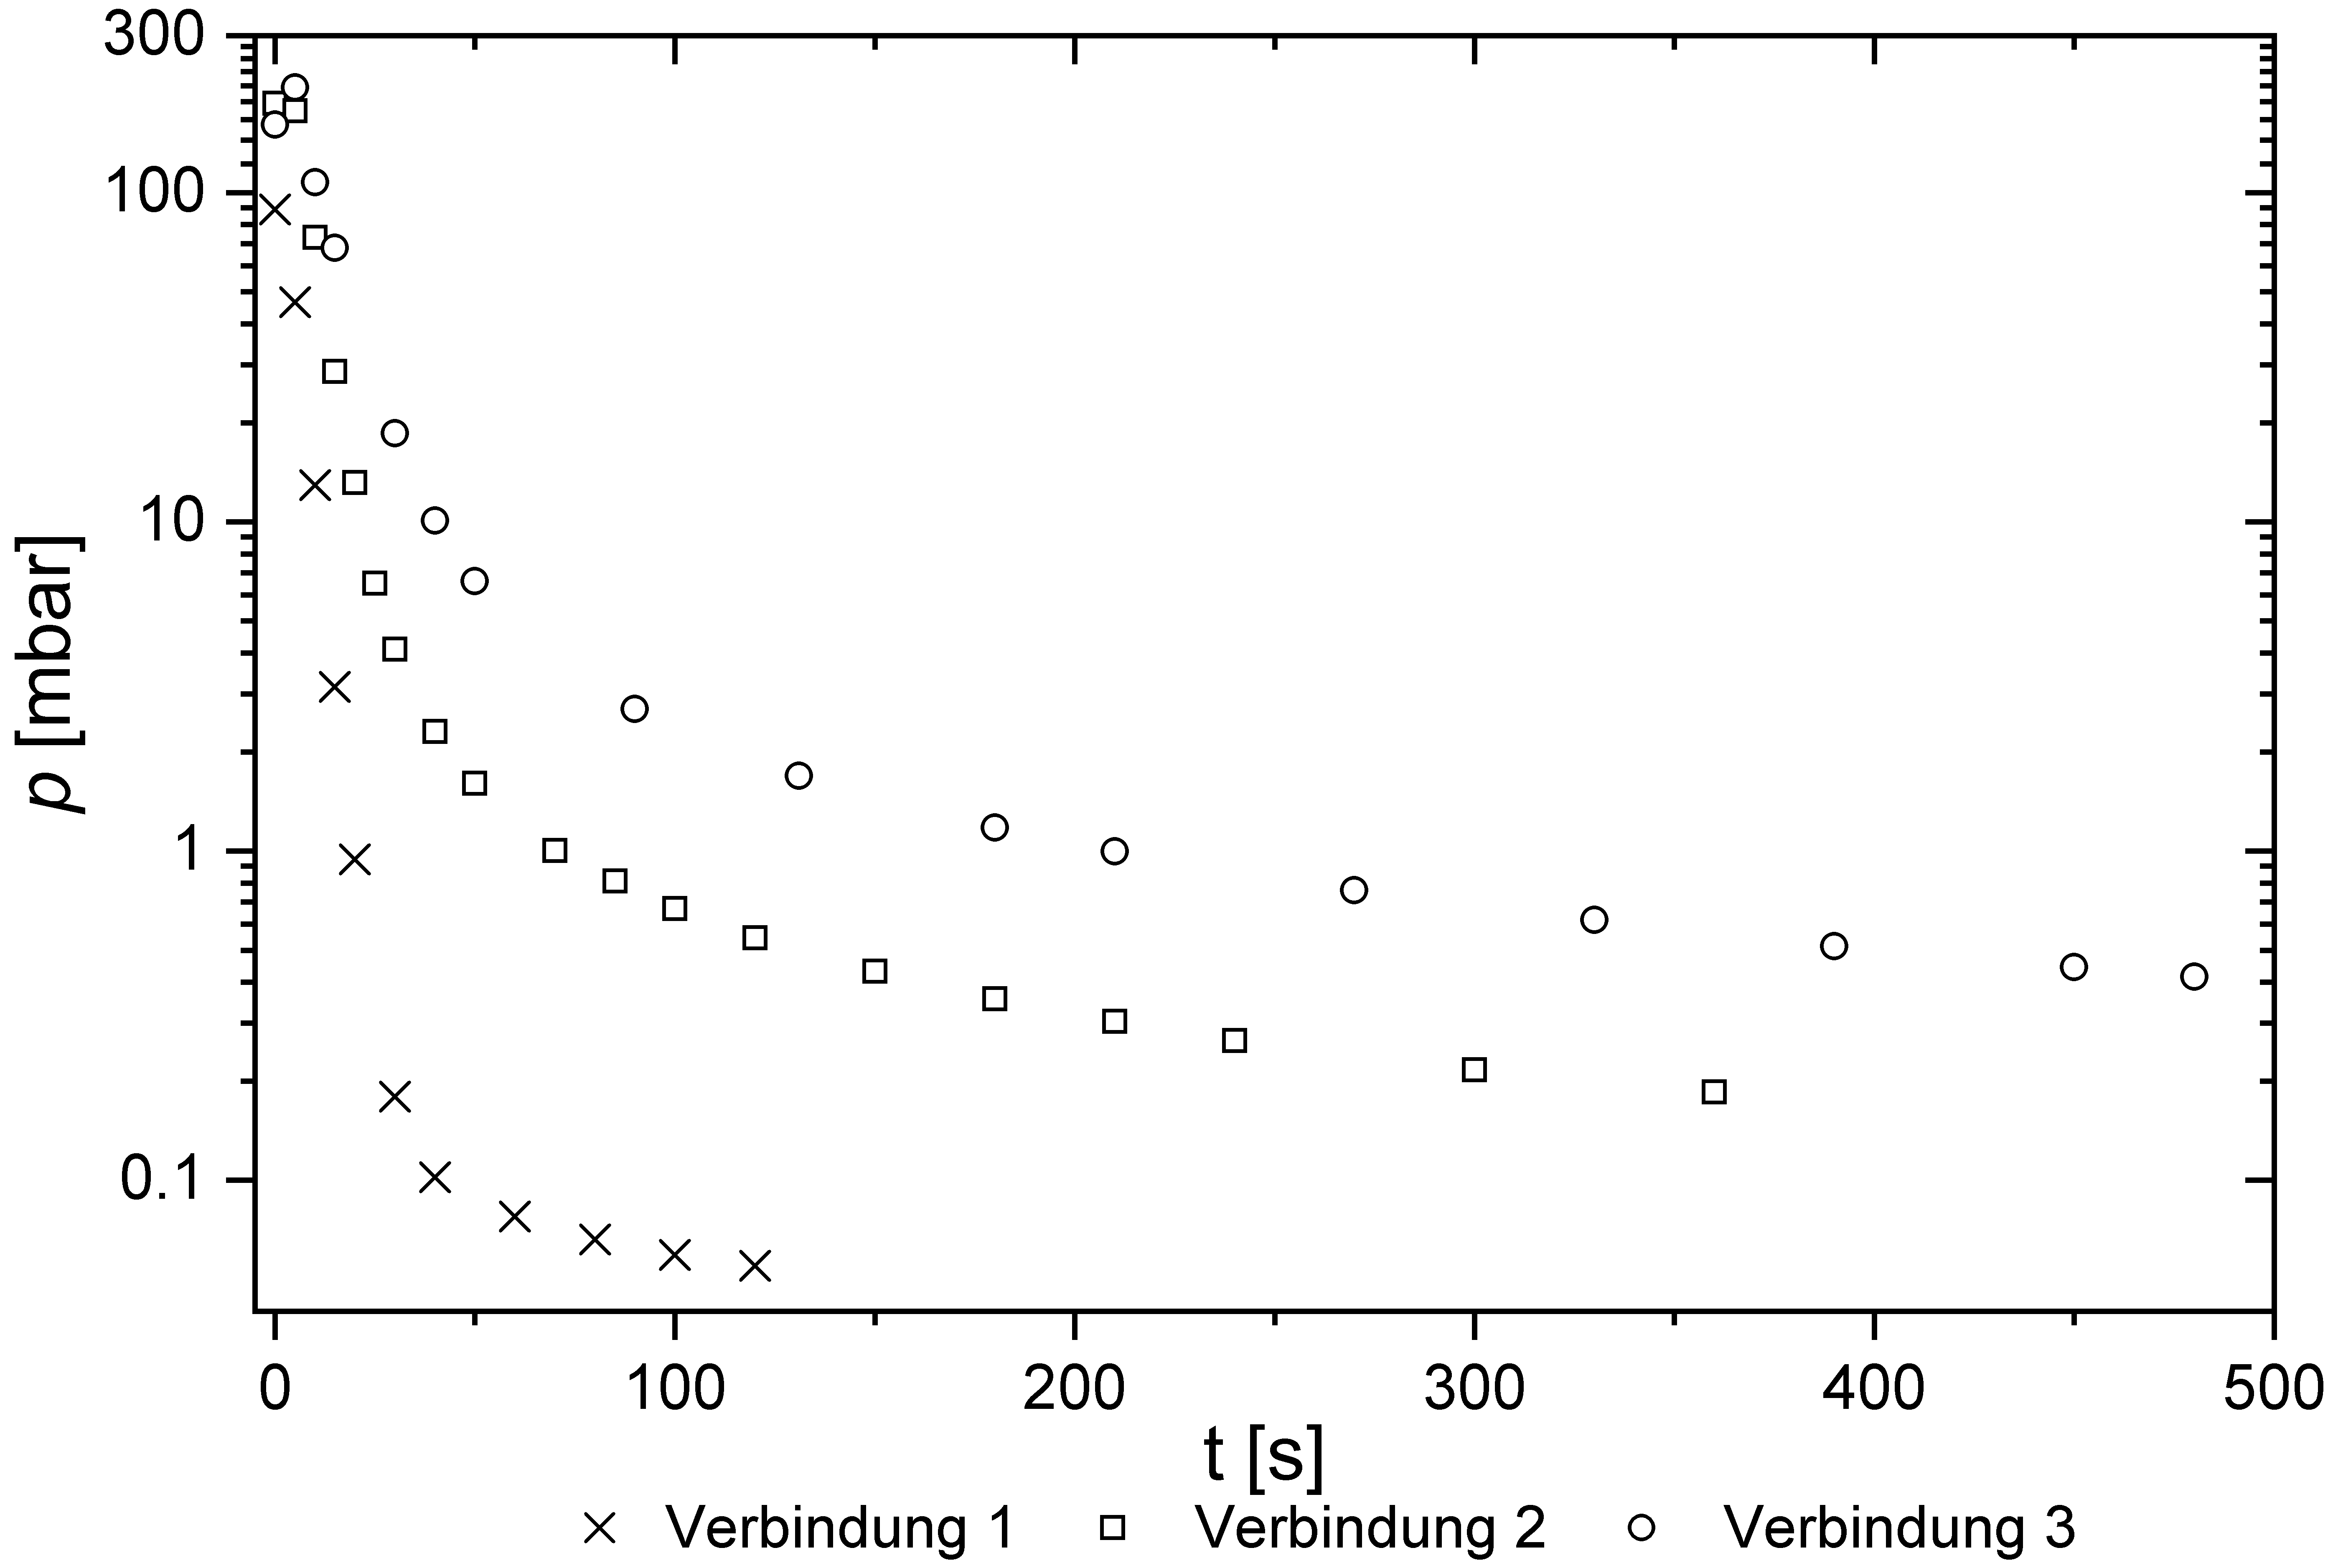
\includegraphics[width=110mm]{graphs/saug1.png}
                \caption{
                    Darstellung von $p$ gegen der Pumpdauer $t$. Man beachte hierbei die logarithmische Auftragung von $p$. Bei den drei verschiedenen Verbindungen handelt es sich um: \textbf{1} Schlauch mit Durchmesser d = 25 mm und Länge $l$ = 65 cm, \textbf{2} Schlauch und Kapillare mit $d$ = (2,0 $\pm$ 0,1) mm und $l$ = (9,5 $\pm$ 0,2) cm, \textbf{3} Schlauch und Kapillare mit $d$ = (3,0 $\pm$ 0,1) mm und $l$ = (9,5 $\pm$ 0,2) cm
                }
                \label{fig:saugEff}
            \end{figure*}
        
            Mithilfe von den Gleichungen \ref{eq:seffExp} und \ref{eq:seffExpM} lassen sich die experimentellen Werte für $S_{eff}$ bestimmen. 
            \\
            Im Folgenden betrachte man nur den Schlauch. Für die molekulare Strömung ergibt sich $\mathbf{S_{eff} = (0,13 \pm 0,11)}$\,$\mathbf{ \frac{m^3}{h}}$ bei einer Steigung von $\kappa = 0,012$. Für die viskose Strömung ergibt sich $\mathbf{S_{eff} = (2,2 \pm 1,28)}$\,$\mathbf{ \frac{m^3}{h}}$ mit $p_0 = 5$ hPa, $t = 40$\,$s$ und $\kappa = 0,244$.\\
            Nun betrachte man den Schlauch mit einer 3 mm Kapillare. Für die molekulare Strömung ergibt sich $\mathbf{S_{eff} = (0,031 \pm 0,037)}$\,$\mathbf{\frac{m^3}{h}}$ mit $x = 0,0029$. Für die viskose Strömung ergibt sich $\mathbf{S_{eff} = (0,76 \pm 0,45)}$ \, $\mathbf{ \frac{m^3}{h}}$ mit $p_0 = 5$\, $hPa$, $t = 65$\,$s$ und $\kappa = 0,095$.
            Die verwendeten Werte wurden in den verschiedenen Graphen in Abbildung \ref{fig:saugEff} abgelesen. Die systematische Unsicherheit des Rezipienten verursacht die teilweisen sehr großen Unsicherheiten. 
            \\
            Um einen Vergleich zu dem experimentell bestimmten effektiven Saugvermögen zu erhalten, lässt sich dieses auch theoretisch berechnen. Aufgrund der unterschiedlichen Druckbereiche, müssen die Leitwerte sowohl für molekulare als auch für die viskose Strömung berechnet werden. Dabei wird Gleichung \ref{eq:lvs} für die viskose Strömung und Gleichung \ref{eq:leitwert} für molekulare Strömung verwendet. Die Ergebnisse der theoretischen Leitwerte befinden sich in Tabelle \ref{tab:theoleit}.
            \begin{table}
                %\centering
                \begin{tabular}{c|c|c|c}
                    \multicolumn{1}{c}{} & \multicolumn{1}{c}{$d$ [mm]} & \multicolumn{1}{c}{$l$ [cm]} & \multicolumn{1}{c}{$L$ [$\frac{m^3}{h}$]}\\
                    \cmidrule(lr){2-2}\cmidrule(lr){3-3}\cmidrule(lr){4-4}
                    \toprule
                     molek.  & $(25,00 \pm 0,50)$    & $(65,00 \pm 1,00)$   & $(10,45 \pm 0,79)$ \\
                                & $(2,00 \pm 0,10)$     & $(9,50 \pm 0,20)$     & $(0,367 \pm 0,006)$\\
                                & $(3,00 \pm 0,10)$     & $(9,50 \pm 0,20)$     & $(1,24 \pm 0,01)$\\
                    \cline{1-4}
                     viskos     & $(25,00 \pm 0,50)$    & $(65,00 \pm 1,00)$   & $(1458,77 \pm 197,50)$\\ %(1,43496 \pm 0,10548)
                                & $(2,00 \pm 0,10)$     & $(9,50 \pm 0,20)$     & $(4,09 \pm 0,11)$\\
                                & $(3,00 \pm 0,10)$     & $(9,50 \pm 0,20)$     & $(20,70 \pm 0,40)$\\
                    \bottomrule
                \end{tabular}
                \caption{Theoretische Ergebnisse mit Unsicherheiten des Leitwertes unter Betrachtung der drei verschiedenen Verbindungen.}
                \label{tab:theoleit}
            \end{table}
            \\
            Nun kann über die Formel \ref{eq:seff} das effektive Saugvermögen im viskosen und molekularen Bereich für die verschiedenen Versuchsaufbauten berechnet werden. Die Ergebnisse mit Unsicherheiten werden in Tabelle \ref{tab:theoseff} zu den Drücken \SI{3,9}{\hecto\pascal} und \SI{0,7}{\hecto\pascal} aufgeführt.\\
            
            \begin{table}
                \centering
                \begin{tabular}{c|c|c}
                    \multicolumn{1}{c}{Konfiguration} & \multicolumn{1}{c}{$S_{eff}$[$\frac{m^3}{h}$] bei $p = 3,9 hPa$} & \multicolumn{1}{c}{$S_{eff}$[$\frac{m^3}{h}$] bei $p = 0,7 hPa$} \\
                    \cmidrule(lr){1-1}\cmidrule(lr){2-2}\cmidrule(lr){3-3}\cmidrule(lr){4-4}
                    \toprule
                     1  & $(4,61 \pm 0,71)$    & $(2,16 \pm 0,11)$   \\
                     2           & $(2,17 \pm 0,19)$     & $(0,314 \pm 0,007)$     \\
                     3          & $(3,77 \pm 0,49)$     & $(0,79 \pm 0,02)$     \\
                    \bottomrule
                \end{tabular}
                \caption{Theoretische Ergebnisse mit Unsicherheiten des effektiven Saugvermögens. Konfiguration 1 beschreibt nur den Schlauch, Konfiguration 2 Schlauch mit \SI{2}{\milli\metre} Kapillare und Konfiguration 3 Schlauch mit \SI{3}{\milli\metre} Kapillare.}
                \label{tab:theoseff}
            \end{table}
        
        
    \section{Diskussion}\label{sec:discussion}
        \subsection{Kalibrierkurve}
            Bei Betrachtung der der Abbildung \ref{fig:calibration}, lässt sich diese in drei verschiedene Bereiche aufteilen. Im Bereich oberhalb von $P_E$ ist verhältnismäßig viel Druck vorhanden, weshalb die mittlere freie Weglänge der Moleküle sehr kurz ist. Aufgrund dessen, kommen Kollisionen sehr häufig vor. Es tritt Konvektion auf. Bei der Wechselwirkung der Stöße der Moleküle mit dem Draht des Pirani-Vakuummeter, wird an diesen umso mehr Energie abgegeben, je höher der Druck ist. Da der Draht somit immer mehr erhitzt wird, bzw. Wärme aufnimmt, bildet sich eine parabelförmige Kennlinie mit absteigender Steigung. Somit handelt es sich um den Bereich mit einer druckunabhängigen Wärmeleitung.
            Wie in den in Kapitel \ref{sec:method} aufgeführten Gleichungen, ist ein linearer Zusammenhang zwischen Druck und Leistung erkennbar. Dies tritt im Bereich zwischen $P_A$ und $P_E$ auf. Eine druckproportionale Wärmeleitung ist hierbei erkennbar.
            Aufgrund der sehr großen mittleren freien Weglänge der Moleküle bei sehr geringen Druck, ist die Wärmeleitung im Bereich unter $P_A$ vernachlässigbar. Korrekte Messungen können aufgrund des seltenen Wechselwirken der Moleküle mit dem Pirani-Vakuummeter nicht mehr gewährleistet werden. Eine asymptotische Linie, mit druckabhängiger Steigung, bildet sich.
            \\
            Eine Kalibrierung des Pirani-Vakuummeter ist somit in dem Bereich über $P_E$, sowie unterhalb von $P_A$ nur mit großen Ungenauigkeiten möglich.
            
        \subsection{Das Saugvermögen der Pumpe}
            Betrachtet man die Ergebnisse aus Tabelle \ref{tab:saug} wird erkennbar, dass die Saugleistung der Pumpe bei abnehmenden Druck geringer wird. Das ist sinnvoll, da bei einem hohen Druck mehr Gasteilchen vorhanden sind im vergleich zu niedrigen Drücken.\\
            Vergleicht man die Ergebnisse nun mit der Firmenangabe fällt auf, dass bei einem Druck von \SI{3,9}{\hecto\pascal} die Saugleistung mehr als \SI[per-mode=fraction]{3,7}{\cubic\metre\per\hour} beträgt. Die Firmenangabe wird auch nicht von der Unsicherheit beinhaltet. Das errechnete Saugvermögen bei einem Druck von \SI{1}{\hecto\pascal} ist geringer als die Angabe und wird ebenfalls nicht von der Unsicherheit beinhaltet.\\
            Es ist jedoch naheliegend, dass bei einem Druck zwischen \SI{1}{\hecto\pascal} und \SI{3,9}{\hecto\pascal} eine Saugleistung von \SI[per-mode=fraction]{3,7}{\cubic\metre\per\hour} ungefähr erreicht wird. Es kann sein, dass die Firmenangabe ein gemittelter Wert über ein bestimmtes Druckintervall ist und aufgrund zu weniger Messdaten und einem anderen Intervall nicht von den experimentell gewonnen Werten erreicht wird. Das ist nur eine Spekulation, da nicht bekannt ist, wie der Hersteller seine Werte zur Berechnung der Angabe ermittelt hat. 
        
        \subsection{Das effektive Saugvermögen der Pumpe}
            Vergleicht man die experimentell gewonnen Werte mit den theoretischen fällt eine große Diskrepanz auf. Die Unterschiede können mit der nicht vorteilhaften Wahl der Drücke bei der Ermittlung des Saugvermögens zusammenhängen. Zudem kann die Wahl der Steigung $\kappa$ zu großen Fehlern führen.
            
    
    \section{Zusammenfassung}\label{sec:conclusion}
            Diese Versuche haben sich relativ simpel durchführen lassen. Es fällt jedoch auf, dass für eine korrekte Datenanalyse mehr und besser gewählte Messwerte nötig sind. Im Allgemeinen ist der Versuchsaufbau mit vielen Unsicherheiten verbunden. Dabei treten die größten Unsicherheiten bei der Kalibrierung des Manometers auf. Dies fiel vor allem im Kapitel \ref{subsec:saug} auf. Hierbei wären größere Druckabstände der 4 verschiedenen Messungen von Nöten gewesen.
        
        
        
    % References
    \bibliographystyle{mnras}
    \bibliography{Ausarbeitung.bib}
    


    % Appendix
    \appendix
    \section{Fehlerrechnung}\label{subsec:fehler}
        Bei der Kalibrierung kann es aufgrund des schnell ansteigenden Stromes am Anfang zu Ablesefehler gekommen sein. Der Strom wurde mit einem Multimeter gemessen, dass ebenfalls eine Unsicherheit hat. Das Pirani-Vakuummeter selbst hat wahrscheinlich eine systematische Unsicherheit bei der Angabe des Druckes. Diese hätte man im Datenblatt des Gerätes nachlesen müssen.\\
        Die Unsicherheiten der theoretischen Leitwerte sind systematischer Natur und wurden mittels linearer Addition fortgepflanzt \citep{fehler}. Für die molekulare Strömung wurde die Unsicherheit folgendermaßen bestimmt. 
        \begin{equation}
            \owncount
                \Delta L = 3600s\cdot\left( \left|\Delta d \cdot 121 \frac{m}{s} \cdot \frac{3d^2}{l}\right| + \left|\Delta l \cdot 121 \frac{m}{s} \cdot \frac{d^3}{-l^2}\right| \right)
            \label{eq:errorml}
        \end{equation}\\
        Hierbei ist $\Delta d$ und $\Delta l$ jeweils die systematische Unsicherheit des Durchmessers bzw. der Länge.\\
        Die folgende Gleichung wurde für die Ermittlung der Unsicherheit der viskosen Strömung verwendet.
        \begin{equation}
            \owncount
                \Delta L = \frac{3600s\cdot\pi}{128\eta}\cdot\left(\left|\Delta d \cdot \frac{4d^3}{l}\cdot \overline{p}\right| + \left|\Delta l \cdot \frac{d^4}{(-l)^2}\cdot \overline{p}\right| + \left|\Delta\overline{p}\cdot\frac{d^4}{l}\right|\right)
            \label{eq:errorvl}
        \end{equation}\\
        Vom Betreuer wurde $\overline{p} = 500$ hPa  angegeben. Da es den mittleren Druck des Gases beschreibt, sollte dieser Wert nicht als konstant angenommen werden. Hier wurde mit einer Abweichung von $\Delta\overline{p} = 0,2 hPa$ gerechnet.\\
        Die Unsicherheit des Saugvermögens beinhaltet Unsicherheiten von statistischer und systematischer Natur. Die statistische Unsicherheit kommt vom mehrmaligen messen der Zeit und dem einstellen des Druckes. Die Unsicherheiten wurden wie folgt fortgepflanzt und dann mittels linearer Addition summiert.
        \begin{equation}
            \owncount
            \begin{aligned}
                \Delta S_{sys} = \left|\Delta p \cdot \left(-\frac{\Delta V}{\Delta t}p_0\right) \left(-\frac{1}{p^2}\right)\right| + \left|\Delta p_0 \cdot \frac{\Delta V}{\Delta t}\left(-\frac{1}{p}\right)\right| \\
                +\left|\Delta V \cdot\frac{1}{\Delta t}\left(-\frac{p_0}{p}\right)\right| + \left|\Delta t \cdot \left(-\frac{\Delta V}{\Delta t^2}\right)\left(-\frac{p_0}{p}\right)\right|
            \end{aligned}
        \end{equation}
        \begin{equation}
            \owncount
            \Delta S_{stat} = \sqrt{\Delta p^2\cdot\left(\frac{\Delta V}{\Delta t}\frac{p_0}{p^2}\right)^2 +\Delta t^2\cdot\left(\frac{\Delta V}{\Delta t^2}\frac{p_0}{p}\right)^2}
        \end{equation}\\
        In der Gleichung der systematischen Unsicherheit wird $\Delta p$ über die Kalibrierkurve ermittelt. Beim Ablesen des Druckes wurde ebenfalls der Strom des Manometers gemessen. Anhand der Schwankung des Multimeters um $\pm 0,4$ mA wurde die Druckunsicherheit für die 4 verwendeten Drücke jeweils aus der Kalibrierkurve abgelesen. Der Außendruck des Versuchsraumes war über den Gesamtzeitraum der Messung wahrscheinlich nicht konstant. Hier wurde mit einem Wert von $p_0 = (960 \pm 50)$ hPa gerechnet. 50 hPa sind in etwa 5\% des Raumdrucks und damit eine gerechtfertigte Wahl der Unsicherheit. Unter der Unsicherheit $\Delta t$ wurde die Reaktionszeit auf etwa 0,4 s angelegt. Für die Wahl der Unsicherheit des Volumens $\Delta V$ wurde ebenfalls etwa 5\% des Ursprungswertes gewählt, also 4 ml. Bei der Gleichung der statistischen Unsicherheiten wurde jeweils die Unsicherheit mittels der Student-t-Verteilung auf einem Vertrauensniveau von 62,8\% berechnet.\\
        Für die Berechnung der Unsicherheit $S_{eff}$ kann für den Schlauch mit Durchmesser \SI{25}{\milli\metre} folgende Formel verwendet werden.
        \begin{equation}
            \owncount
            \begin{aligned}
            \Delta S_{eff} = \left|-\Delta S \cdot \left(\frac{1}{S}+\frac{1}{L}\right)^{-2} \cdot \left(-\frac{1}{S^2}\right)\right| \\
             + \left|-\Delta L\cdot \left(\frac{1}{S}+\frac{1}{L}\right)^{-2}\cdot\left(-\frac{1}{L^2}\right)\right|
            \end{aligned}
        \end{equation}\\
        Für die Konfiguration Schlauch mit Kapillare muss die Unsicherheit mit nachfolgender Formel berechnet werden. 
        \begin{equation}
            \owncount
            \begin{aligned}
            \Delta S_{eff} = \left|\Delta S \cdot \frac{L_S^2L_K^2}{(S(L_S+L_K)+L_KL_S)^2}\right| \\
            + \left|\Delta L_S \cdot \frac{S^2L_K^2}{(S(L_S+L_K)+L_KL_S)^2}\right| \\
            + \left|\Delta L_K \cdot \frac{S^2L_S^2}{(S(L_S+L_K)+L_KL_S)^2}\right|
            \end{aligned}
        \end{equation}\\
        Wobei $L_K$ der Leitwert für die verwendete Kapillare und $L_S$ der Leitwert für den Schlauch ist.\\
       
            

    \label{lastpage}
\end{document}
